\section{1.16b}

\begin{quote}\color{black!80}\slshape
  Use the construction given in \cite[Theorem~1.39]{Sipser} to
  convert the following two nondeterministic automata to equivalent
  deterministic finite automata.

  [\dots]
  
  \begin{center}
    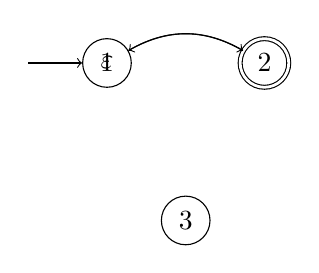
\begin{tikzpicture}
      \node[draw, circle] (I) at (0,0){1} ;
      \node[draw, circle, double, double distance=1pt] (II) at (2,0){2} ;
      \node[draw, circle] (III) at (1,-2){3} ;
      \draw[->] (-1,0) -- (I) ;
      \draw[->] (I) to[bend left] (II) node[midway] {$\varepsilon$} ;
      \draw[->] (II) to[bend right] (I) ;
    \end{tikzpicture}
  \end{center}
  \cite[p.~87]{Sipser}
\end{quote}
